\section{Extreme Values, Critical Points, and Saddle Points}

To find the local extremum of a function in one variable, we look for points on its graph having a horizontal tangent line.
The local extrema are also called \textbf{relative extrema}.

\subsection{Local Extremum}
Let $f(x, y)$ be defined on a region $R$ containing the point $(a, b)$. Then,

\begin{enumerate}
    \item $f(a, b)$ is a \textbf{local maximum} value of $f$ if $f(a, b) \geq f(x, y)$ for all domain points $(x, y)$ in an
    open disk centered at $(a, b)$.

    \item $f(a, b)$ is a \textbf{local minimum} value of $f$ if $f(a, b) \leq f(x, y)$ for all domain points $(x, y)$ in an
    open disk centered at $(a, b)$.
\end{enumerate}

Local maxima correspond to \textit{mountain peaks} on the surface $z = f(x, y)$, whereas local minima correspond to
\textit{valley bottoms}.

\begin{theorem}[First Derivative Test]
    If $f(x, y)$ has a local extremum at an interior point $(a, b)$ of its domain and if the first partial derivatives exist
    there, then $f_x(a, b) = f_y(a, b) = 0$.
\end{theorem}


\subsection{Critical Point}
An interior point of the domain of a function $f(x, y)$ where both $f_x$ and $f_y$ are zero, or where one or both of $f_x$
and $f_y$ do not exist is a \textbf{critical point} of $f$.

\textbf{Theorem 7} essentially says that a function $f(x, y)$ can only assume extreme values at critical points or boundary
points. But not every critical point gives rise to a local extremum. A differentiable function of one variable may have a
\textit{point of inflection}, whereas a differentiable function in two variables might have a \textit{saddle point}.

\begin{example}
    \normalfont Find the local extreme values of $f(x, y) = x^2 + y^2$.

    We find the gradient of the function, $\grad f = \langle 2x, 2y \rangle$. The partial derivatives are 0 at $(0, 0)$.
    Since $f$ is never negative, the origin is the local minimum.
\end{example}


\subsection{Saddle Point}
A critical point $(a, b)$ where in every open disk centered at $(a, b)$, there are domain points where $f(x, y) > f(a, b)$
and domain points where $f(x, y) < f(a, b)$ is called a \textbf{saddle point} $(a, b, f(a, b))$ of the surface
$z = f(x, y)$.

\begin{example}
    \normalfont Find the local extreme values of $f(x, y) = y^2 - x^2$.

    We find that the partial derivatives of $f$ are $f_x = -2x$ and $f_y = 2y$. Both the parital derivatives are 0 at the origin.
    However, note that $f(x, 0) = -x^2 < 0 (for x > 0)$, and $f(0, y) = y^2 > 0 (for y > 0)$. Hence, the origin is a saddle point.
\end{example}

\begin{theorem}[Second Derivative Test]
    Suppose that $f(x, y)$ and its first and second partial derivatives are continuous throughout a disk centered at $(a, b)$, and
    that $f_X(a, b) = f_y(a, b) = 0$. Then
    \begin{enumerate}
        \item $f$ has a \textbf{local maximum} at $(a, b)$ if $f_{xx} < 0$ and $f_{xx}f_{yy} - f{xy}^2 > 0$ at $(a, b)$.
        \item $f$ has a \textbf{local minimum} at $(a, b)$ if $f_{xx} > 0$ and $f_{xx}f_{yy} - f{xy}^2 > 0$ at $(a, b)$.
        \item $f$ has a \textbf{saddle point} at $(a, b)$ if $f_{xx}f_{yy} - f{xy}^2 < 0$ at $(a, b)$.
        \item The test is inconclusive at $(a, b)$ if $f_{xx}f_{yy} - f{xy}^2 = 0$.
    \end{enumerate}
\end{theorem}


\subsection{Discriminant or Hessian of \texorpdfstring{$f$}{f}}
The expression $f_{xx}f_{yy} - f_{xy}^2$ is called the \textbf{discriminant} or \textbf{Hessian} of f.
\begin{equation}
    f_{xx}f_{yy} - f_{xy}^2 =
    \begin{vmatrix}
        f_{xx} & f_{xy} \\ f_{yx} & f_{yy}
    \end{vmatrix}
\end{equation}

\textbf{Theorem 8} essentially says that if the discriminant is positive, the surface curves the same way in all directions.
If $f_{xx} < 0$, then it curves downwards, giving rise to local maxima, and vice-versa. And if the discriminant is negative,
then it curves upwards in some directions and downwards in others.

\begin{example}
    \normalfont Find the local extreme points of $f(x, y) = xy$.

    \begin{figure}[htp]
        \centering
        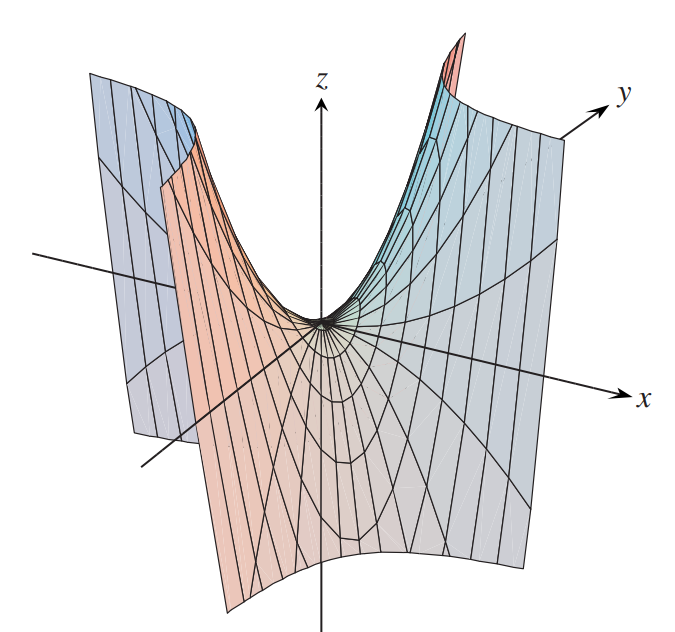
\includegraphics[scale=0.35]{saddle-point.png}
        \caption{The surface $z = xy$}
    \end{figure}

    Since $f$ is differentiable everywhere, its critical points can occur only where
    $$f_x = y = 0 \ \ \ \text{and} \ \ \ f_y = x = 0$$

    This only happens at $(0, 0)$. Next, we find the double partial derivatives
    $$f_{xx} = 0, \ \ \ f_{yy} = 0, \ \ \ f_{xy} = 1$$

    Hence, the discriminant becomes $f_{xx}f_{yy} - f{xy}^2 = -1 < 0$, and hence, the origin is a saddle point.
    Since there are no other critical points, the function does not have a local extremum.
\end{example}


\subsection{Absolute Extrema on Closed Bounded Regions}
Absolute extrema of a continuous function $f(x, y)$ on a closed bounded region $R$ are found in three steps:
\begin{enumerate}
    \item List down the critical points of $f$ and evaluate $f$ at these points.
    \item List down the boundary points of $f$ where it has local maxima/minima and evaluate $f$ at these points.
    \item The maximum value of $f$ in this list is the absolute maxima of $f$ on $R$, and the minimum value is the
    absolute minima.
\end{enumerate}

\begin{example}
    \normalfont Find the absolute maximum and minimum values of $f(x, y) = 2 + 2x + 2y - x^2 - y^2$ on the triangular
    region bounded by $x = 0, y = 0, y = 9 - x$.

    First, we find the critical points of $f$.
    $$f_x = 2 - 2x = 0 \ \ \ \text{ and } \ \ \ f_y = 2 - 2y = 0$$
    which gives the point $(1, 1)$. $f(1, 1) = 4$.

    For the boundary points, we have (for):
    \begin{enumerate}
        \item
        $$y = 0 \implies f(x, 0) = 2 + 2x - x^2$$
        The absolute extrema for this function can occur at its end-points, and in the interior where its derivative is 0.
        $f'(x, 0) = 2 - 2x = 0 \implies x = 1$. \\
        Therefore, $f(0, 0) = 2, f(9, 0) = -61, f(1, 0) = 3$.

        \item
        $$x = 0 \implies f(0, y) = 2 + 2y - y^2$$
        The absolute extrema for this function can occur at its end-points, and in the interior where its derivative is 0.
        $f'(0, y) = 2 - 2y = 0 \implies y = 1$. \\
        Therefore, $f(0, 0) = 2, f(0, 9) = -61, f(0, 1) = 3$.

        \item
        $$y = 9 - x \implies f(x, 9-x) = -61 + 18x - 2x^2$$
        The absolute extrema for this function can occur at the interior points where its derivative is 0.
        $f'(x, 9-x) = 18 - 4x = 0 \implies x = \frac{9}{2}$. \\
        Therefore, $f(\frac{9}{2}, 9-\frac{9}{2}) = -\frac{41}{2}$.
    \end{enumerate}
\end{example}